\documentclass[xcolor=dvipsnames]{beamer}
%
% Choose how your presentation looks.
%
% For more themes, color themes and font themes, see:
% http://deic.uab.es/~iblanes/beamer_gallery/index_by_theme.html
%

\mode<presentation>

\usetheme{Warsaw}      % or try Darmstadt, Madrid, Warsaw, ...\textbf{\(\(\(\)\)\)}}

\usecolortheme{beaver} % or try albatross, beaver, crane, ...
\usefonttheme{professionalfonts}  % or try serif, structurebold, ...
\setbeamertemplate{navigation symbols}{}
\setbeamertemplate{caption}[numbered]
\usepackage{ragged2e}
\usepackage[spanish]{babel}
\usepackage[utf8x]{inputenc}
\usepackage{graphicx}
\usepackage{lmodern}
\usepackage{multicol}
\usepackage{xcolor}
\usepackage{pgf}
\usepackage{textpos}
\usepackage{tikz}
\usepackage{apacite}
\usepackage{natbib}
\usepackage{stackengine}
\usepackage{amsmath}
\usepackage{algorithm2e}
\usepackage{algorithmic}
\usepackage{caption}
\usepackage{graphicx}
\usepackage{subcaption}
\usepackage{multirow}
\captionsetup[subfigure]{font=scriptsize}
\usepackage{mathtools} % for "\mathclap" macro; loads "amsmath" package
\usepackage{ragged2e}


%\newcommand{\figcite}[3]{
  %\def\stackalignment{l}
  %\stackunder{\includegraphics[width=#1]{#2}}{\scriptsize Source: #3}}

\newcommand\tab[1][1cm]{\hspace*{#1}}

\definecolor{myNewColorText}{RGB}{204,0,0}
%\definecolor{myNewColorBack}{RGB}{79,156,69}
\definecolor{myNewColorBack}{RGB}{91,147,195}
\definecolor{myNewColorTittlePanel}{RGB}{216,216,216}


\newcounter{saveenumi}
\newcommand{\seti}{\setcounter{saveenumi}{\value{enumi}}}
\newcommand{\conti}{\setcounter{enumi}{\value{saveenumi}}}

\resetcounteronoverlays{saveenumi}


\title[MIDAS]{Asociación de variantes en regiones codificantes de genes con datos clínicos en pacientes colombianos usando minería de datos.}
\author[Vélez, Jennifer.]{
    Autor: Jennifer Vélez Segura \\
    Director: Elizabeth León Guzmán \\
    Asesor: Claudia Serrano
}

\institute[U. Nacional de Colombia]
{
	Grupo de Investigación -- MIDAS\\   
    Universidad Nacional de Colombia, Bogot\'{a} D.C., Colombia
}
\date{Mayo 2019}

\setbeamercolor{section in toc}{fg=myNewColorBack}

% Change the background and the color of the text
\setbeamercolor*{palette primary}{bg = myNewColorBack, fg = myNewColorText}
\setbeamercolor*{palette secondary}{fg = myNewColorText}
\setbeamercolor*{palette tertiary}{fg = myNewColorText}
\setbeamercolor*{palette quaternary}{fg = myNewColorText}
\setbeamercolor{titlelike}{parent=structure,bg=myNewColorTittlePanel}


% Setup the bibliography
\setbeamertemplate{bibliography entry title}{}
\setbeamertemplate{bibliography entry location}{}
\setbeamertemplate{bibliography entry note}{}

%\setbeamercolor{block title}{fg=myNewColorText, bg=myNewColorBack}

% Change the color bullets of TOC
\setbeamercolor{section number projected}{bg=myNewColorBack,fg=myNewColorText}
\setbeamercolor{subsection number projected}{bg=myNewColorBack}
\setbeamercolor*{item}{fg=myNewColorBack}

% Change the size of font TOC
%%%%%%%%%%%%%%%%%%%%%%%%%%%%%% User specified LaTeX commands.
%Two column ToC
\setbeamerfont{section in toc}{size= \scriptsize}
\setbeamerfont{subsection in toc}{size= \scriptsize}

% image directory
\graphicspath{ {images/} }

\logo{\pgfputat{\pgfxy(0.3,-0.5)}{\pgfbox[right,base]{
\includegraphics[height=1.2cm ]{midas_logo.png}}}}

\begin{document}

\begin{frame}
  \titlepage
\end{frame}

\begin{frame}{Contenido}
    \begin{columns}[onlytextwidth,T]
        \begin{column}{.55\textwidth}
	            \tableofcontents[sections=1-3]
        \end{column}
        \begin{column}{.60\textwidth}
            \tableofcontents[sections=4-]
        \end{column}
    \end{columns}
\end{frame}

\section{Introducción}
\subsection{Secuenciación}
\begin{frame}{Contenido}
    \begin{columns}[onlytextwidth,T]
        \begin{column}{.55\textwidth}
            \tableofcontents[currentsection, sections=1-3]
        \end{column}
        \begin{column}{.60\textwidth}
            \tableofcontents[currentsection, sections=4-]
        \end{column}
    \end{columns}
\end{frame}


\begin{frame}{Secuenciación}	
	\justifying
	La secuenciación es el proceso químico que permite identificar el orden de nucleótidos en molécula de ADN, ARN o una proteína \cite{Kulski2016}.

	\centering 
	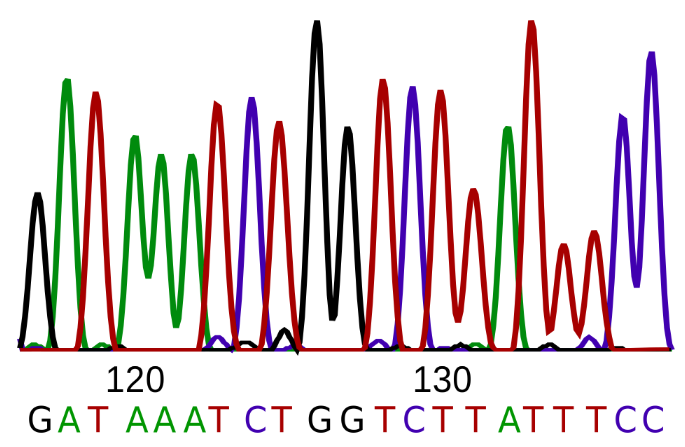
\includegraphics[width=60mm]{secuenciacion}
	
	\hfill \break
	
	\justifying
	\tiny{Tomado de: https://experiment.com/u/v0RZUQ}
\end{frame}

\begin{frame}{Secuenciación}
	
	El proceso de secuenciación se realiza a través de los siguientes pasos:
	
	\begin{itemize}
		\item Extracción de ADN.
		\item Secuenciación de la muestra de ADN.
		\item Obtención de lecturas.
		\item Análisis de genes.
		\item Generación de reportes.
	\end{itemize}
	
\end{frame}

\begin{frame}{Secuenciación de siguiente generación (NGS)}	
	\justifying
	Se han desarrollado diferentes metodologías para realizar secuenciación, estas son conocidas como secuenciación de alto rendimiento y tienen la capacidad de realizar secuenciaciones de manera masiva, rápida y económica  \cite{Kulski2016}. 
	
\hfill \break
	\centering
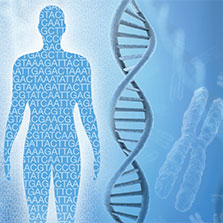
\includegraphics[width=25mm]{ngs.jpg}

\hfill \break

\justifying
\tiny{https://www.almacgroup.com/news/almac-group-to-collaborate-with-illumina-on-next-generation-sequencing-based-companion-diagnostic-development/}
	
\end{frame}

\begin{frame}{Secuenciación con Illumina}
	\centering
	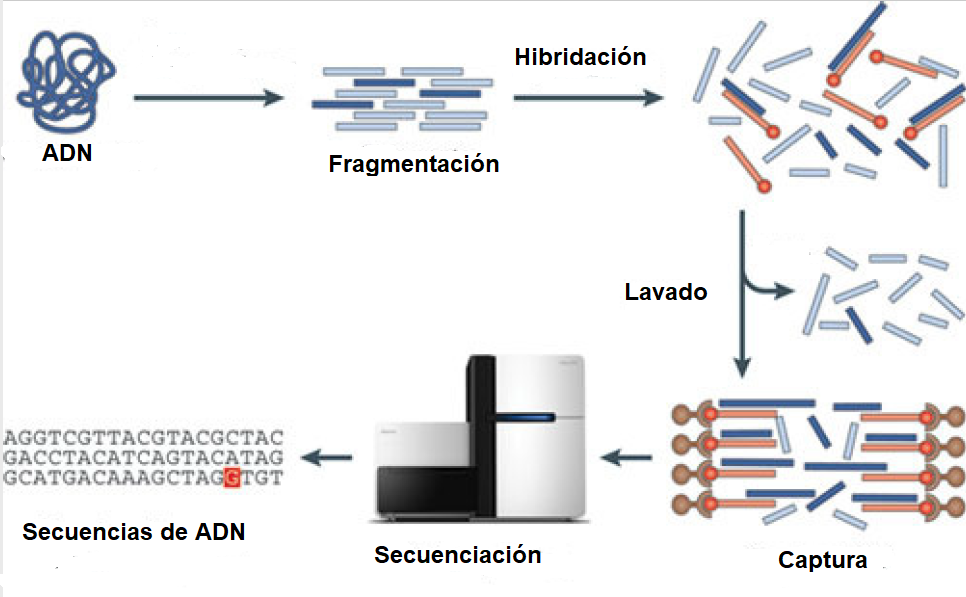
\includegraphics[width=11cm]{secuenciacion1.png}
\end{frame}

\subsection{Alineamiento}


\begin{frame}{Alineamiento}
	\justifying
	Es el proceso de mapear las lecturas secuenciadas usando un genoma de referencia, que para humanos generalmente es el hg19.
	\hfill \break
	
	\begin{figure}
	\centering
	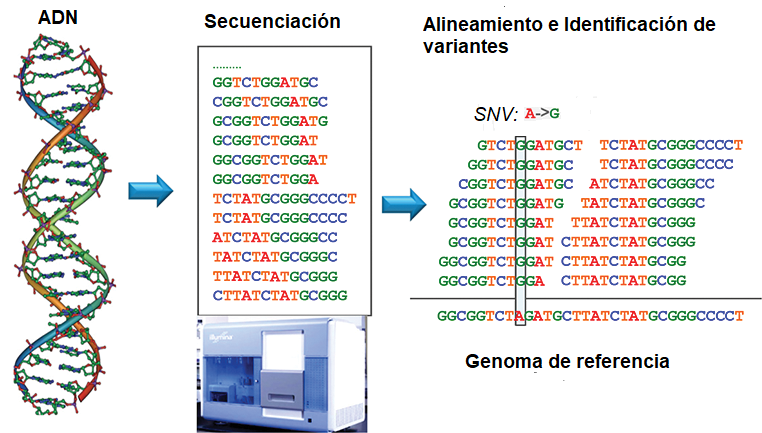
\includegraphics[width=8cm]{resumenngs.png}
	\end{figure}
\justifying
\tiny{https://www.intechopen.com/books/cloud-computing-architecture-and-applications/}	
\end{frame}

\subsection{Variantes}
\begin{frame}{Variantes}
	\begin{figure}
		\centering
		\begin{subfigure}[b]{0.47\textwidth}
			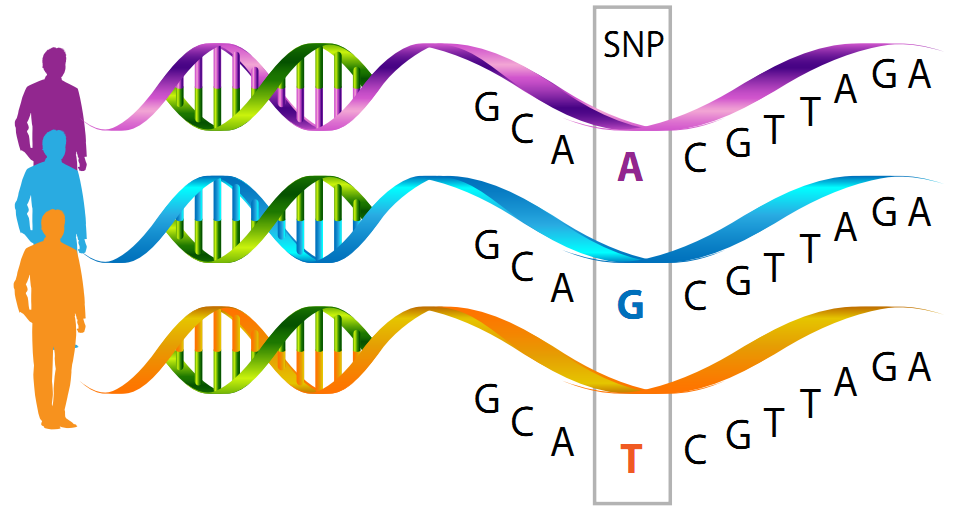
\includegraphics[width=\textwidth]{snp.png}
			\caption{Variante de Nucleótido Simple SNV}
		\end{subfigure}
		~ %add desired spacing between images, e. g. ~, \quad, \qquad, \hfill etc. 
		%(or a blank line to force the subfigure onto a new line)
		\begin{subfigure}[b]{0.47\textwidth}
			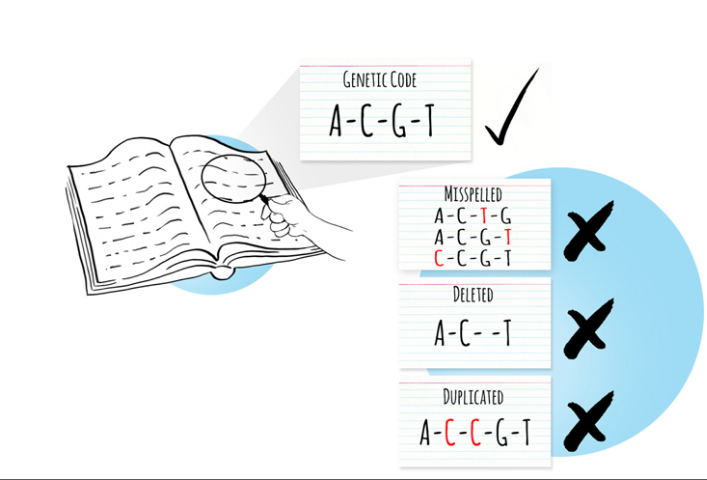
\includegraphics[width=\textwidth]{variante.png}
			\caption{ Variantes Indels}
		\end{subfigure}
		\caption{Tipos de variantes según el cambio de núcleotido}
	\end{figure}
	
\end{frame}

\begin{frame}{Retos de análisis de secuencias}

\begin{enumerate}
	\justifying
	\item No existe un protocolo \textit{``gold stardard"} para realzar un análisis de secuencias.
	
	\item Existe una gran cantidad de información obtenida que no es posible de analizar sin utilizar métodos computacionales.
	
	\item La población colombiana no cuenta con estudios de este tipo y no se encuentra caracterizada como otras poblaciones.
	
	\item En la mayoría de los estudios realizados no cuentan con la información clínica.
\end{enumerate}

   
\end{frame}

\subsection{Objetivos}

\begin{frame}{Objetivos}
	
	\begin{block}{}
		{\justifying 
			Proponer un modelo de minería de datos que permita asociar variantes con características clínicas de pacientes colombianos.
		}
	\end{block}
	
	\begin{itemize}
		\item Realizar la identificación de variantes en pacientes colombianos.
		\item Integrar la información clínica con las variantes obtenidas.
		\item Proponer un modelo de minería.
		\item Validar y visualizar los resultados del modelo de minería
	\end{itemize}
		
\end{frame}

\section{Integración de datos}
\subsection{Datos}

\begin{frame}{Datos}

\begin{block}{Origen de los datos}
	{\justifying 
		Los datos utilizados en el presente trabajo proviene de la información clínica de 228 pacientes colombianos, distribuidos en 133 pacientes femeninas y 95 pacientes masculino secuenciados en regiones codificantes de 4813 genes. 
	}
\end{block}

\textit{Estos datos fueron donados por el Laboratorio Genetix S.A.S.}
\end{frame}

\begin{frame}{Flujo de trabajo}
\begin{figure}
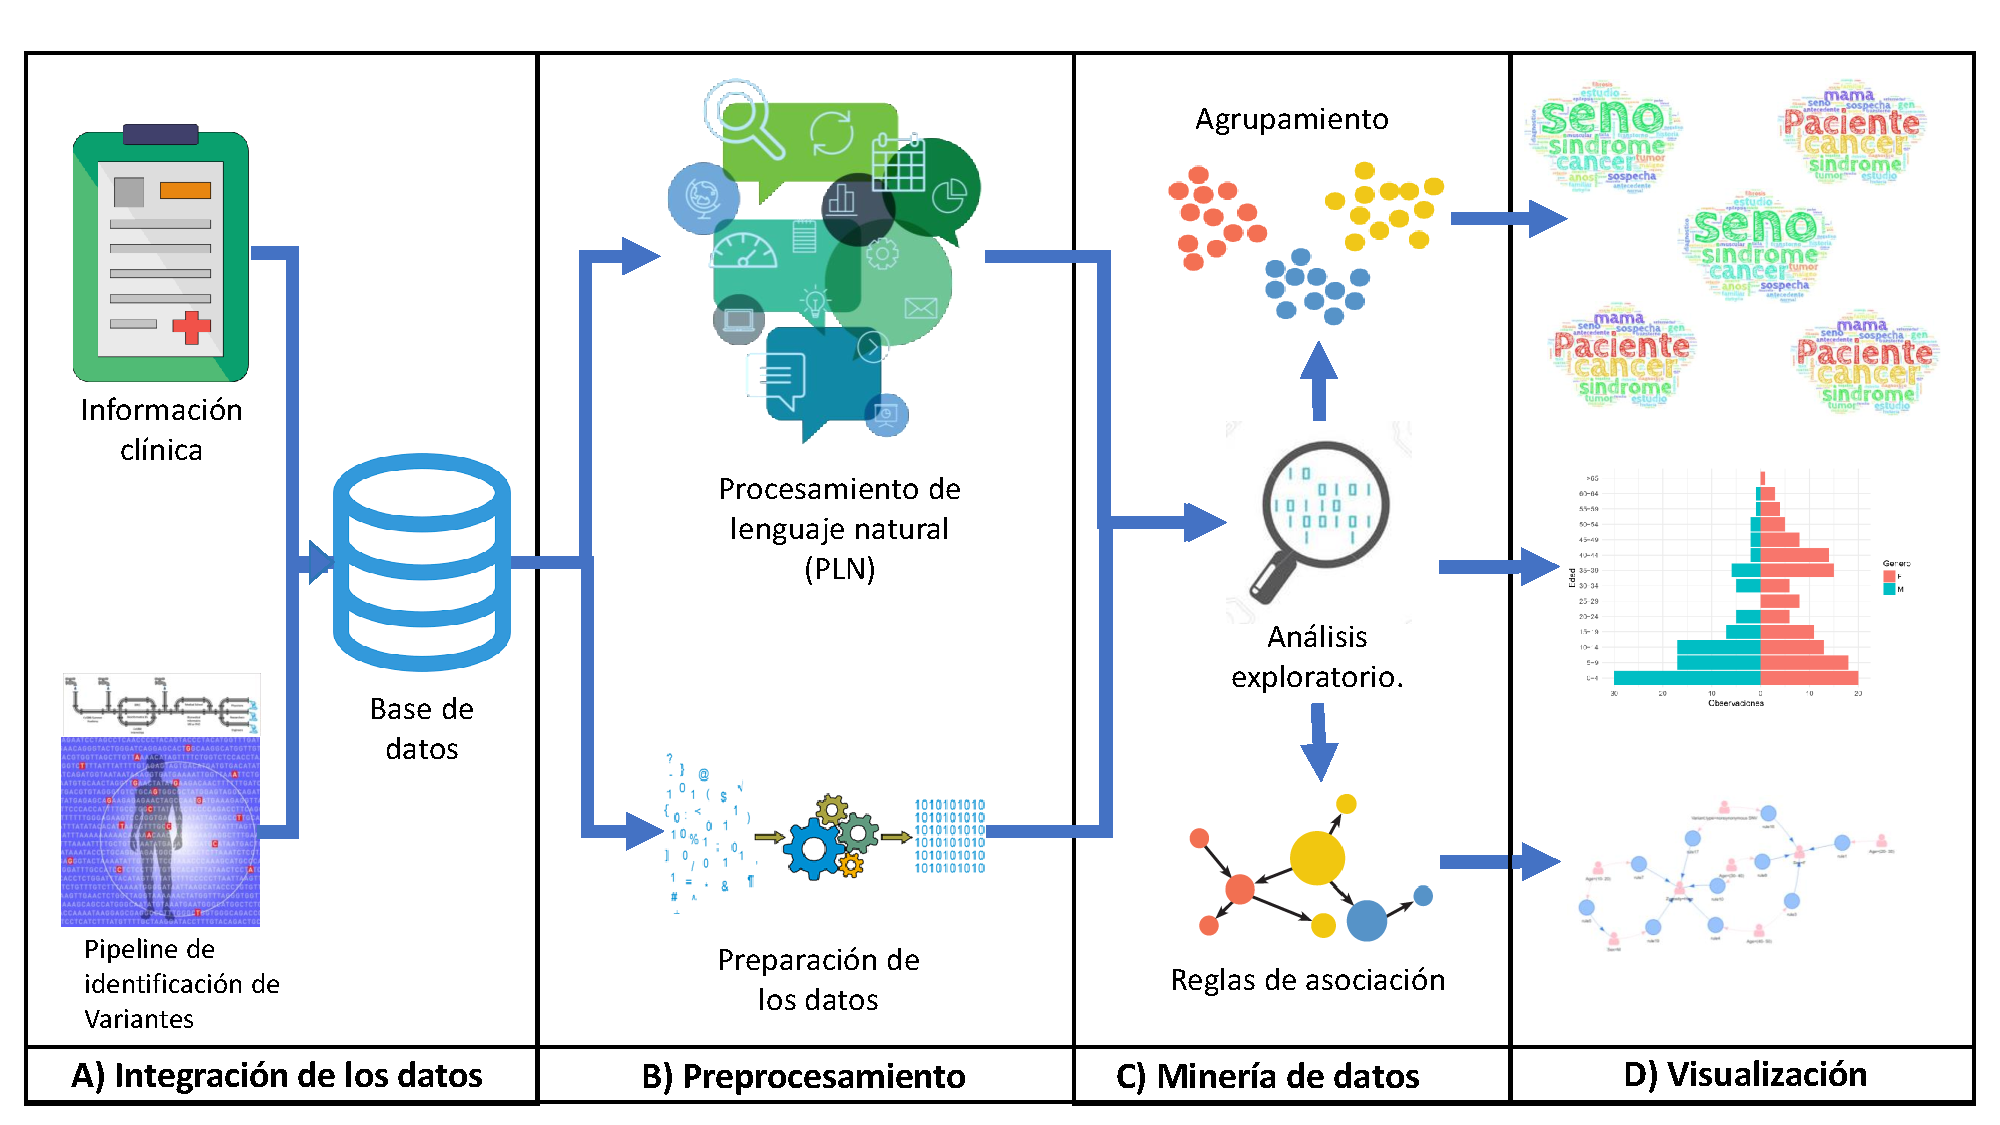
\includegraphics[width=1\textwidth]{KDDtesis.pdf}
\end{figure}
\end{frame}


\subsection{Identificación de variantes}

\begin{frame}{Calidad de la secuenciación}
	\begin{figure}
		\centering
		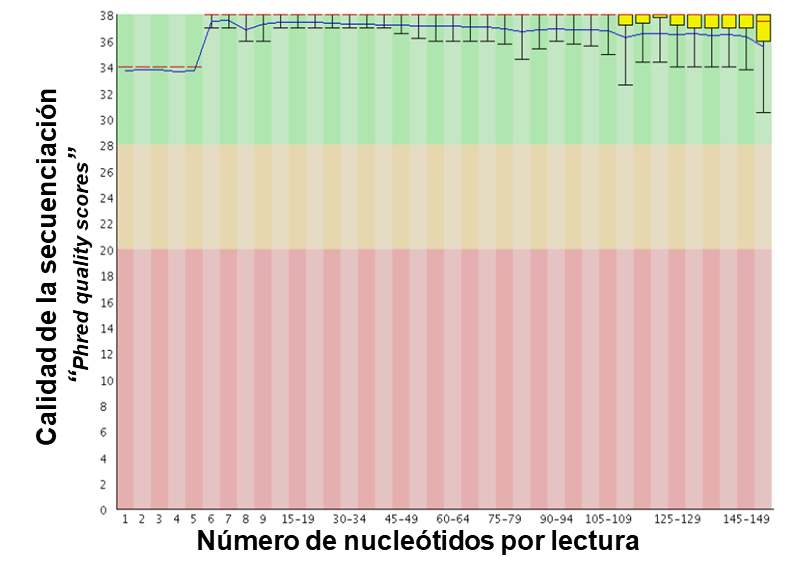
\includegraphics[width=0.8\linewidth]{calidadfastq.png}
		\label{fig:fastq2}
	\end{figure}
\end{frame}


\begin{frame}{Identificación de variantes}
	\justifying 
	Los pipelines bioinformáticos para NGS son comúnmente desarrollados en una plataforma especifica y pueden ser adaptados según las necesidades del laboratorio, la mayoría de los pipelines consisten en los siguientes pasos \cite{Roy2018}:
	\justifying 
	\begin{enumerate}[1.]
		\justifying
		\item Generación de secuencias.
		\item Alineamiento de las secuencias.
		\item Llamado de variantes.
		\item Filtrado de variantes.
		\item Anotación de variantes.
		\item Priorización de variantes. 
	\end{enumerate}
\end{frame}

\begin{frame}{Pipeline implementado en un cluster}
	
	\begin{figure}
		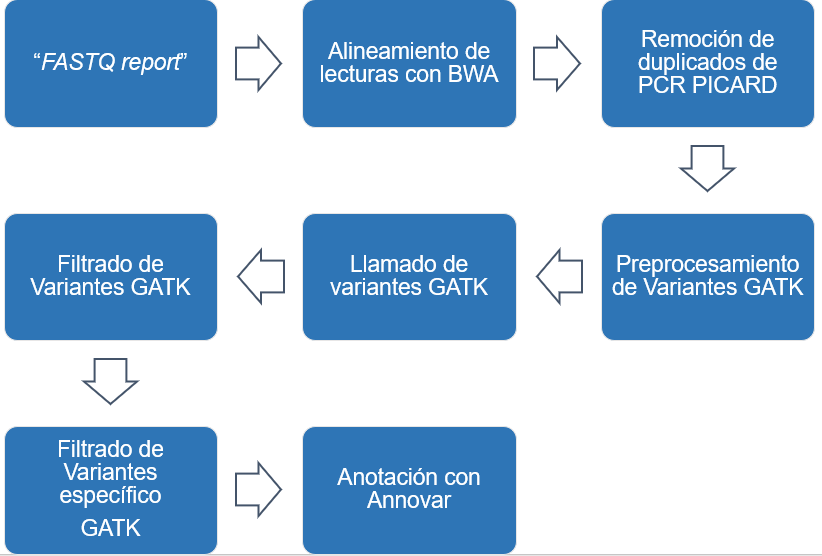
\includegraphics[width=1\textwidth]{pipeline1}
		
	\end{figure}
	
\end{frame}


\begin{frame}{Validación}
	
	\begin{enumerate}[1.]
		\item Validación con datos internos. Datos de un paciente con 4813 genes(Illumina).
		\item Validación con datos públicos. Datos del exoma completo NA12878.
	\end{enumerate}
	\centering
	
\includegraphics[width=30mm]{validacion.png}
	
\end{frame}

\begin{frame}{Validación datos internos}
\begin{table}[h!]
	\centering
	\footnotesize
	\begin{table}[]
		\begin{tabular}{l|l|l|l|l|}
			\cline{2-5}
			& \multicolumn{4}{c|}{\textbf{Variantes}} \\ \cline{2-5} 
			& SNV    & Indels  & Desconocida  & Total \\ \hline
			\multicolumn{1}{|l|}{Pipeline}   & 54538  & 8855    & 122          & 63515 \\ \hline
			\multicolumn{1}{|l|}{Calibradas} & 10425  & 828     & 44           & 11297 \\ \hline
			\multicolumn{1}{|l|}{Illumina}   & 9601   & 436     & 28           & 10065 \\ \hline
		\end{tabular}
	\end{table}
	\caption{Resultados de variantes obtenidas}
\end{table}
\end{frame}

\begin{frame}{Validación con datos internos}
	\begin{figure}[]
		\centering
		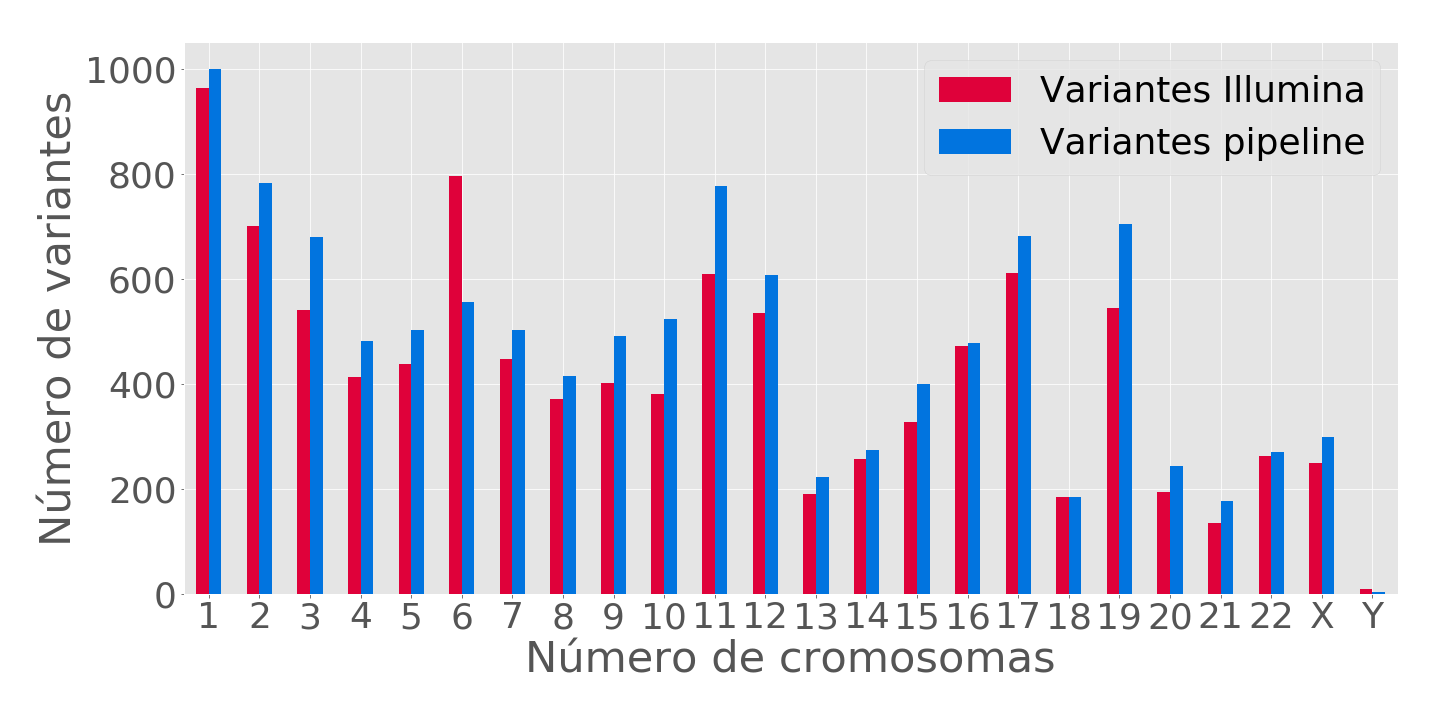
\includegraphics[width=1\textwidth]{validacion1}
		\caption{Distribución de variantes a lo largo de los cromosomas} \label{fig:distribucion}
	\end{figure}
\end{frame}

\begin{frame}{Validación con el exoma NA12878}
\begin{table}[H]
	\centering  
	\begin{tabular}{l|l|l|l|}
		\cline{2-4}
		& \multicolumn{3}{c|}{\textbf{Variantes Exoma}} \\ \cline{2-4} 
		& SNV           & Indels         & Total        \\ \hline
		\multicolumn{1}{|l|}{Pipeline} & 30893         & 3324           & 34217        \\ \hline
		\multicolumn{1}{|l|}{Públicas} & 29749         & 3101           & 32850        \\ \hline
	\end{tabular}
	\caption{Tabla de Variantes obtenidas a partir de un exoma}
	\label{tabla:tabla2}
\end{table} 
\end{frame}

\begin{frame}{Validación exoma NA12878}
\begin{figure}[H]
	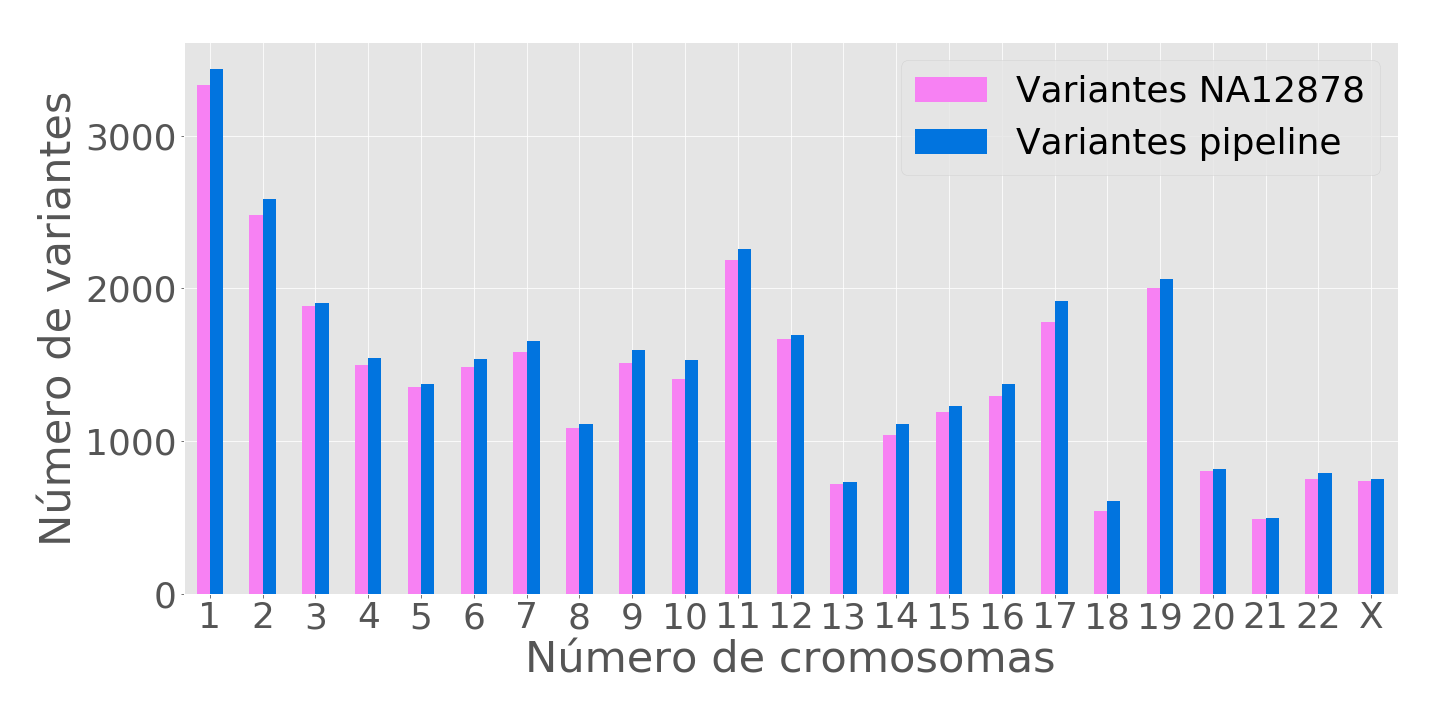
\includegraphics[width=1\textwidth]{validacion2.png}
	\caption{Distribución de variantes a lo largo de los cromosomas para los exomas} \label{fig:tabla2}
\end{figure}
\end{frame}


\begin{frame}{Validación exoma NA12878}
    \begin{table}[H]
	    \begin{center}
		    \begin{tabular}{|l|l|}
			    \hline 
			    \textbf{TP} &  \textbf{TN} \\
			    \hline 
			    32110 & 0  \\ \hline
			    \textbf{FP} &  \textbf{FN} \\
			    \hline
			    1033 &  0\\ \hline
		    \end{tabular}
		\caption{Matriz de confusión}
		\label{tabla:tabla3}
	\end{center}
\end{table}


\begin{table}[H]
	\begin{center}
		\begin{tabular}{|l|l|l|}
			\hline 
			\textbf{Sensibilidad} & \textbf{Especificidad} & \textbf{PPV} \\
			\hline 
			96.88 & 100 & 100 \\ \hline
		\end{tabular}
		\caption{Análisis de sensibilidad y especificidad}
		\label{tabla:tabla4}
	\end{center}
\end{table}

\end{frame}

\begin{frame}{Variante en el Exoma NA1278}
	
	chr10,96541616,96541616,G,A,exonic,CYP2C19
	
\begin{figure}[H]
	\centering
	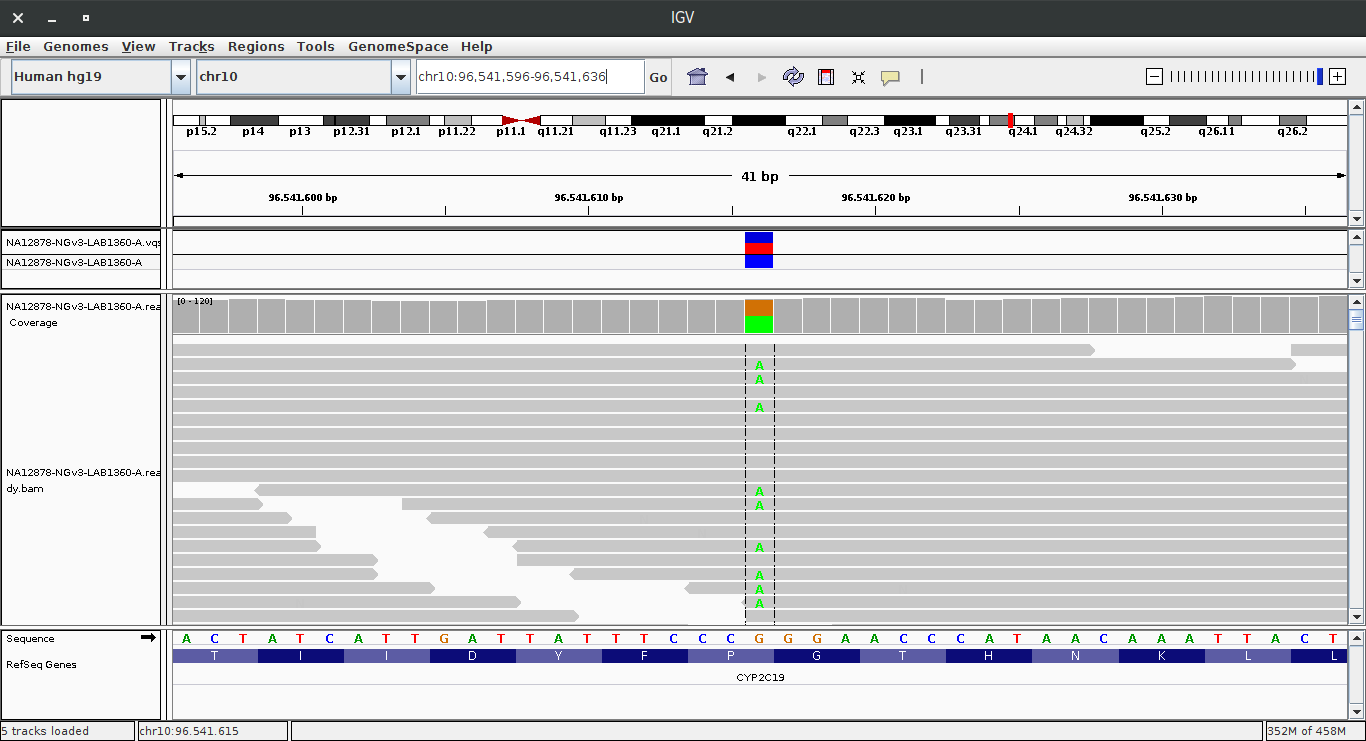
\includegraphics[width=1\textwidth]{IGV}
\end{figure}
\end{frame}

\subsection{Modelo de datos}

\begin{frame}{Contenido}
    \begin{columns}[onlytextwidth,T]
        \begin{column}{.55\textwidth}
            \tableofcontents[currentsection, sections=1-3]
        \end{column}
        \begin{column}{.60\textwidth}
            \tableofcontents[currentsection, sections=4-]
        \end{column}
    \end{columns}
\end{frame}

\begin{frame}{Modelo de datos}
    
    \begin{itemize}
    	\item Autenticación de grupos.
    	\item Autenticación de usuarios.
    	\item Permisos de usuario.
    	\item Migraciones de Django 
    	\item Administración de Django.
    	\item Secciones de Django.	 	
    \end{itemize}
    
\end{frame}

\begin{frame}{Modelo de datos}
      \begin{figure}
		\centering
		\begin{subfigure}[b]{0.2\textwidth}
			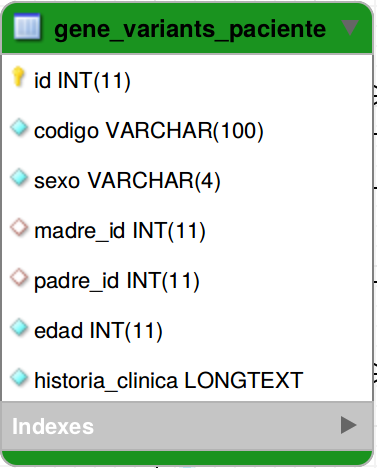
\includegraphics[width=\textwidth]{tabla1.png}
			\caption{Datos de los pacientes}
		\end{subfigure}
		\quad
		~ %add desired spacing between images, e. g. ~, \quad, \qquad, \hfill etc. 
		%(or a blank line to force the subfigure onto a new line)
		\begin{subfigure}[b]{0.2\textwidth}
			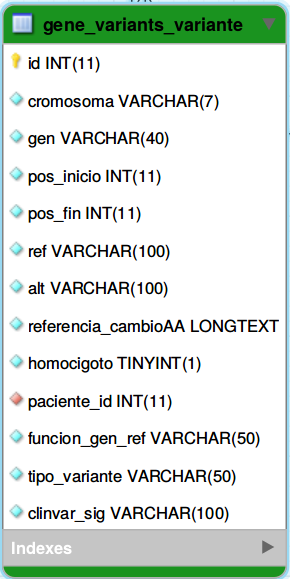
\includegraphics[width=\textwidth]{tabla2.png}
			\caption{Información de variantes}
		\end{subfigure}
		\caption{Gestión de variantes e información clínica}
	\end{figure}
\end{frame}
    

\begin{frame}{Interfaz de consulta}
	\begin{figure}
		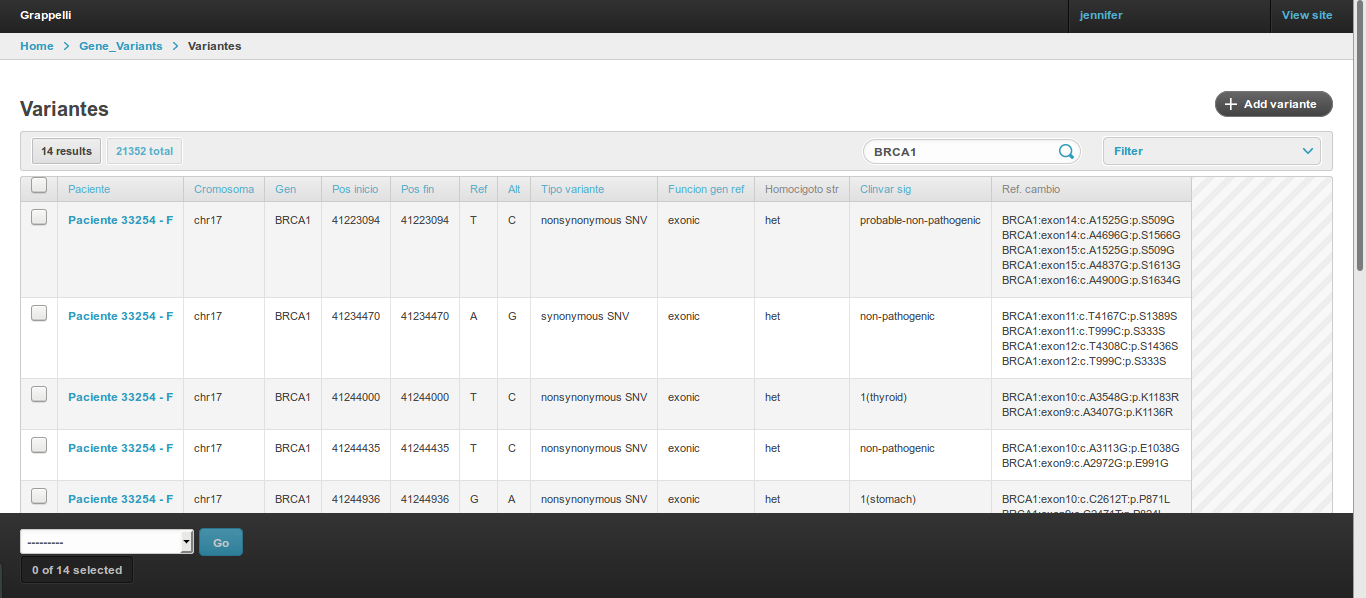
\includegraphics[width=\textwidth]{consulta}
		\caption{Ejemplo de consulta por gen}
	\end{figure}
\end{frame}
\section{Minería de datos}
\subsection{Preprocesamento}
    \begin{frame}{Contenido}
    \begin{columns}[onlytextwidth,T]
        \begin{column}{.55\textwidth}
            \tableofcontents[currentsection, sections=1-3]
        \end{column}
        \begin{column}{.60\textwidth}
            \tableofcontents[currentsection, sections=4-]
        \end{column}
    \end{columns}
\end{frame}


\begin{frame}{Preprocesamiento de la información clínica}
   	\begin{enumerate}[1.]
   	
		\justifying 
		\item  Digitalización de la información clínica y carga a la base de datos.
		\item Remoción de \textit{``stop words''} en español, tildes y caracteres especiales como la letra ñ y todos los documentos se unificaron en letras minúsculas.
		\item Creación de un diccionario de sinónimos, donde se reemplazaron palabras que hacen referencia a una misma característica, teniendo en cuenta la interpretación clínica. \item Cálculo de la frecuencias de palabras dentro de los documentos. 
		\item Remoción de las palabras pam, pacientes, secuenciación y gen dado que no son un factor diferenciador de los documentos.  
	   	\end{enumerate}

\end{frame}

\begin{frame}{Procesamiento de lenguaje natural}
	
   \begin{figure}
		\centering
		\begin{subfigure}[b]{0.4\textwidth}
			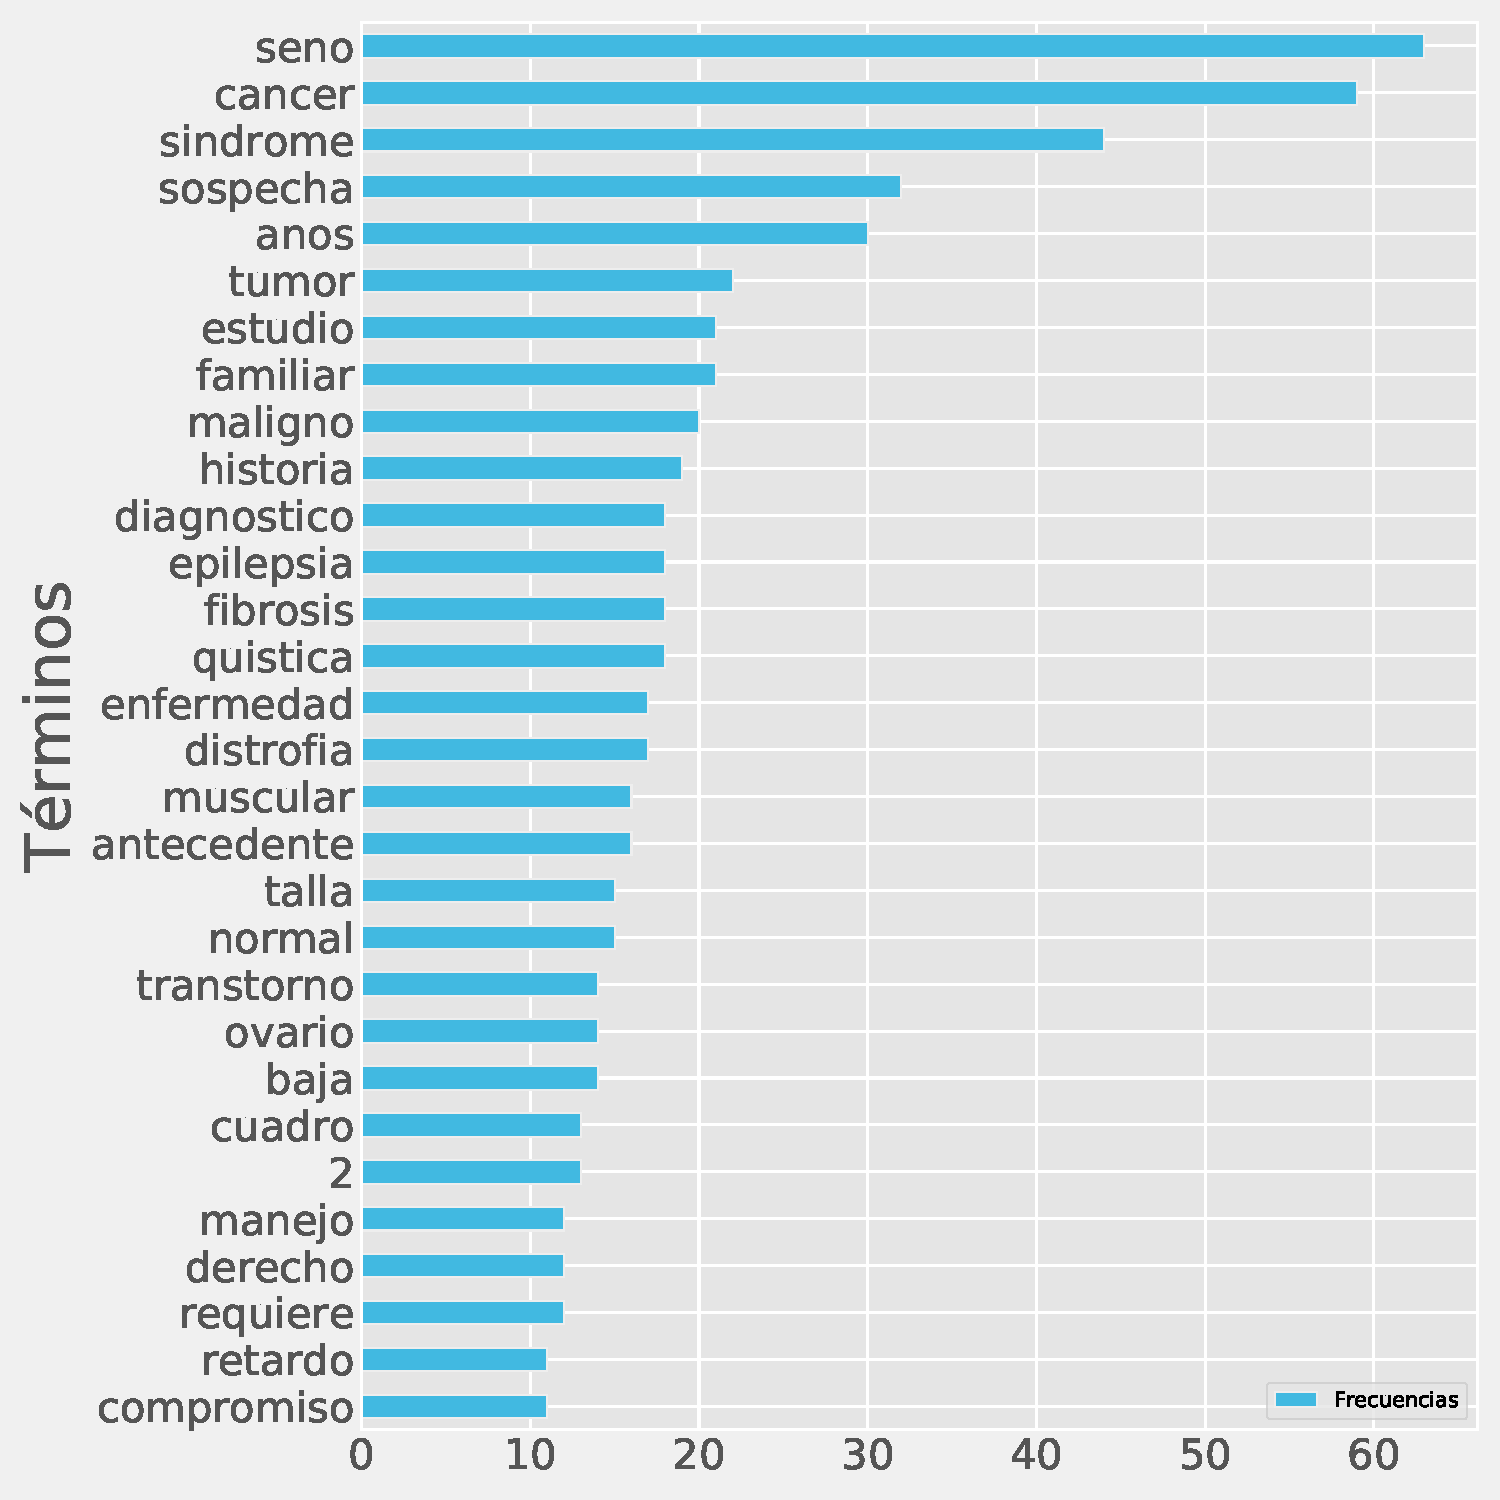
\includegraphics[width=\textwidth]{frecuecias.pdf}
			\caption{Frecuencia de términos}
		\end{subfigure}
		~ %add desired spacing between images, e. g. ~, \quad, \qquad, \hfill etc. 
		%(or a blank line to force the subfigure onto a new line)
		\begin{subfigure}[b]{0.47\textwidth}
			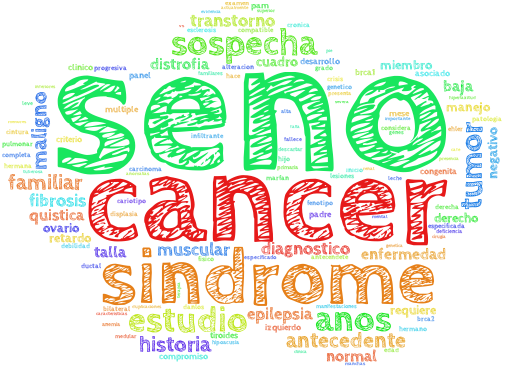
\includegraphics[width=\textwidth]{sin_stop.png}
			\caption{Frecuencia de palabras}
		\end{subfigure}
		\caption{Representación de términos frecuentes.}
	\end{figure}
\end{frame}

\begin{frame}{Preprocesamiento de lenguaje natural}
	\begin{figure}[H]
		\centering
		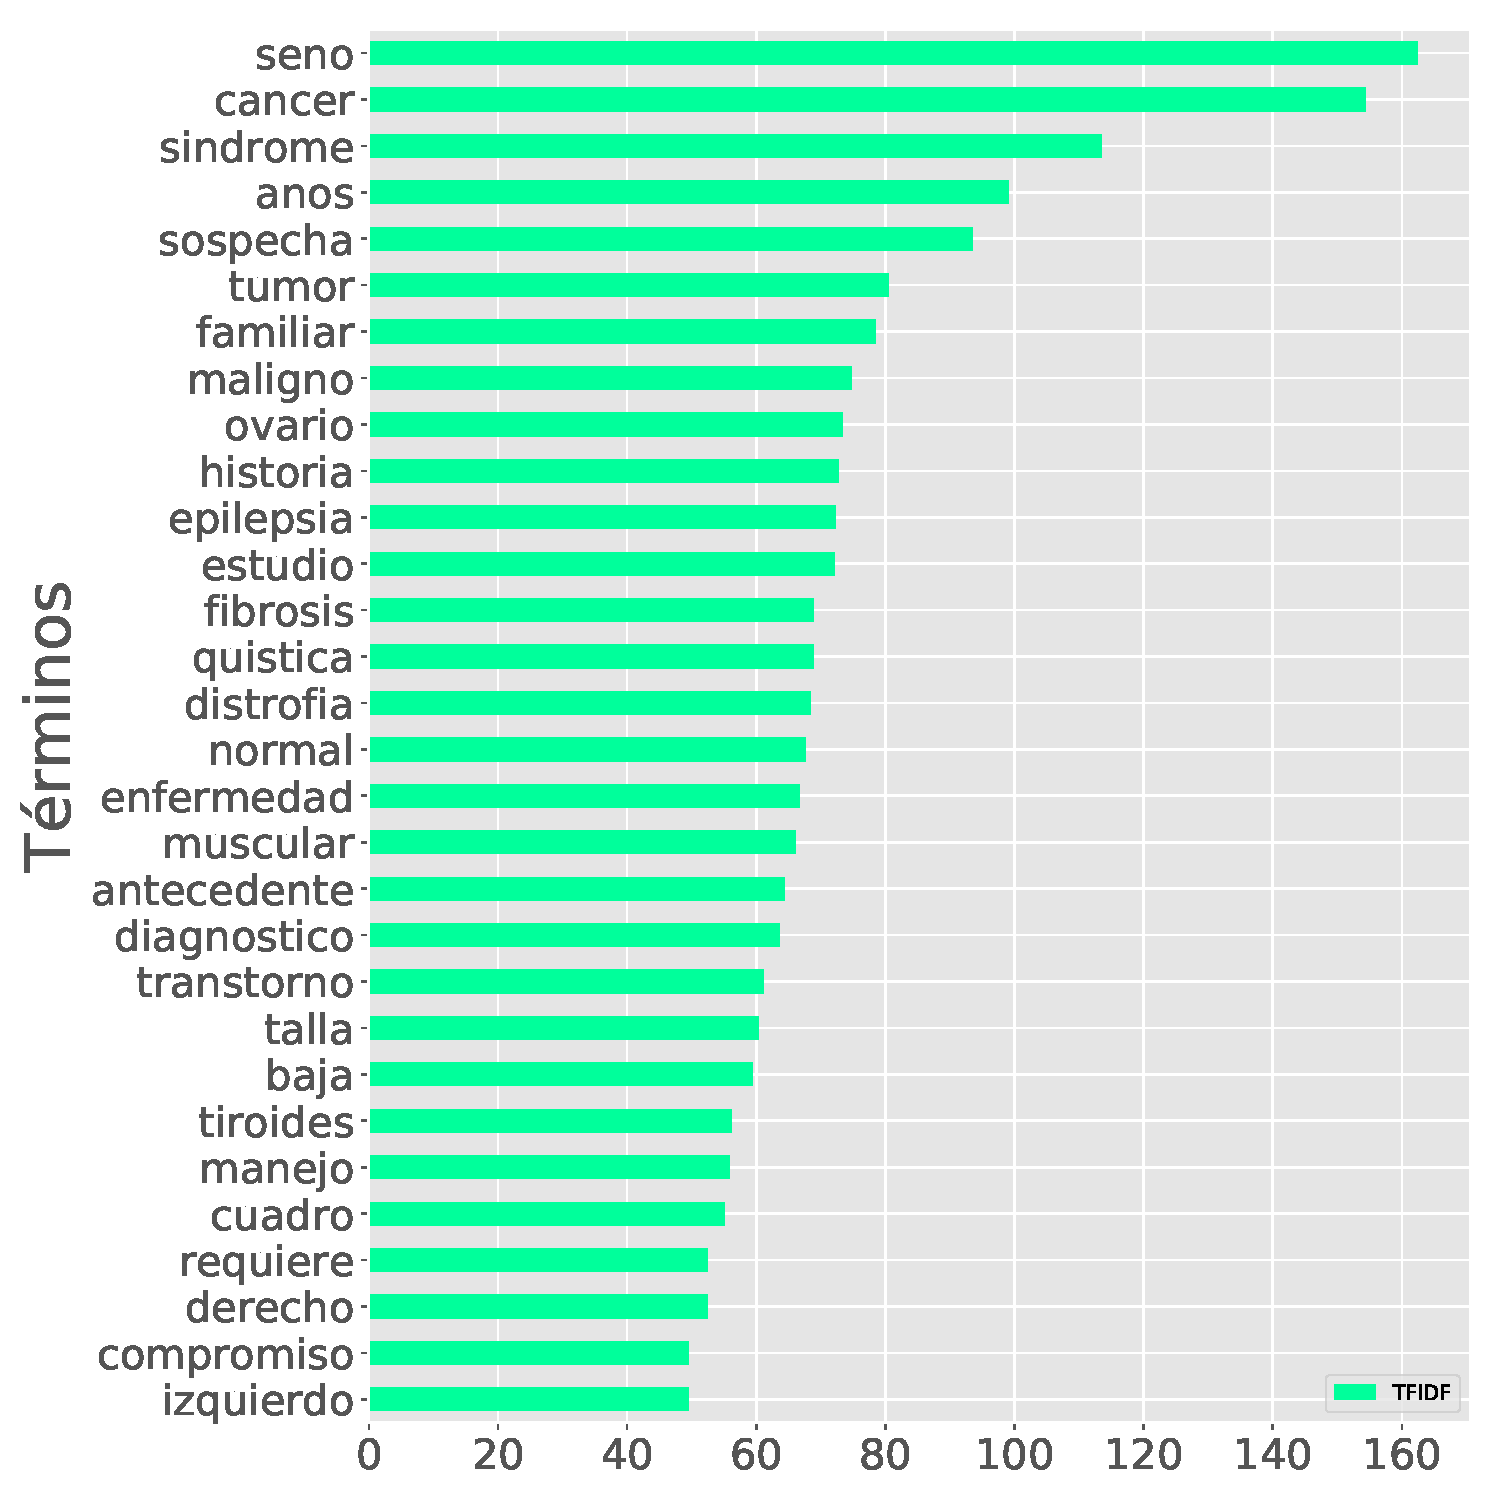
\includegraphics[width=0.5\textwidth]{tfidf.pdf}
		\centering
		\caption{TF-IDF.} \label{fig:idf}
	\end{figure}
\end{frame}

\begin{frame}{Agrupamiento de la información clínica}
 \begin{figure}
		\centering
		\begin{subfigure}[b]{0.5\textwidth}
			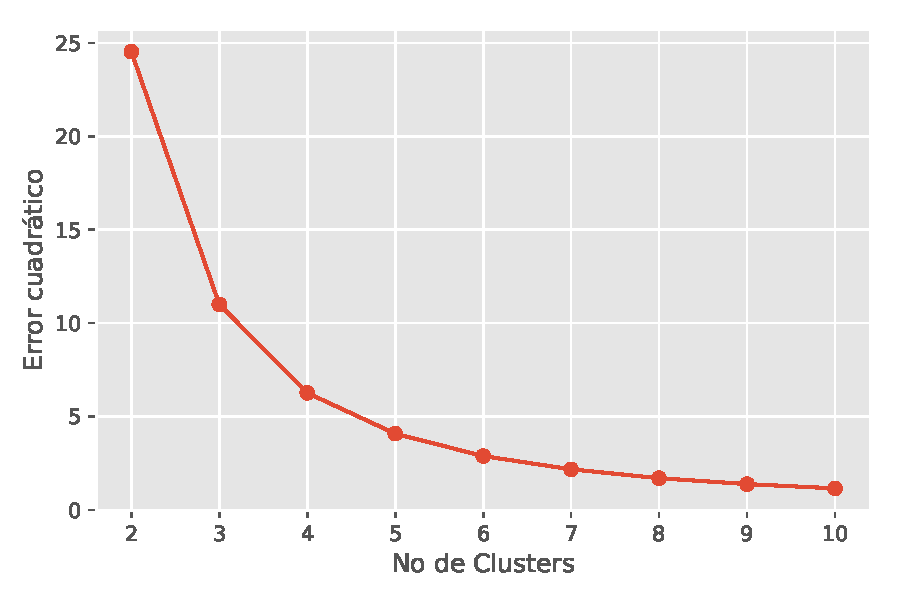
\includegraphics[width=\textwidth]{Clusters.pdf}
			\caption{Error cuadrático}
		\end{subfigure}
		~ %add desired spacing between images, e. g. ~, \quad, \qquad, \hfill etc. 
		%(or a blank line to force the subfigure onto a new line)
		\begin{subfigure}[b]{0.35\textwidth}
			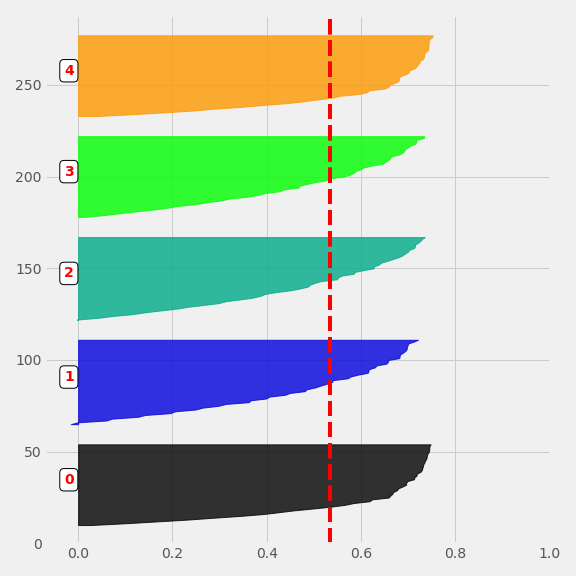
\includegraphics[width=\textwidth]{S.png}
			\caption{ Valor Silhouette}
		\end{subfigure}
		\caption{Medidas de selección de número de grupos}
	\end{figure}
\end{frame}

\begin{frame}{Agrupamiento de la información clínica}
 \begin{figure}[H]
		\centering
		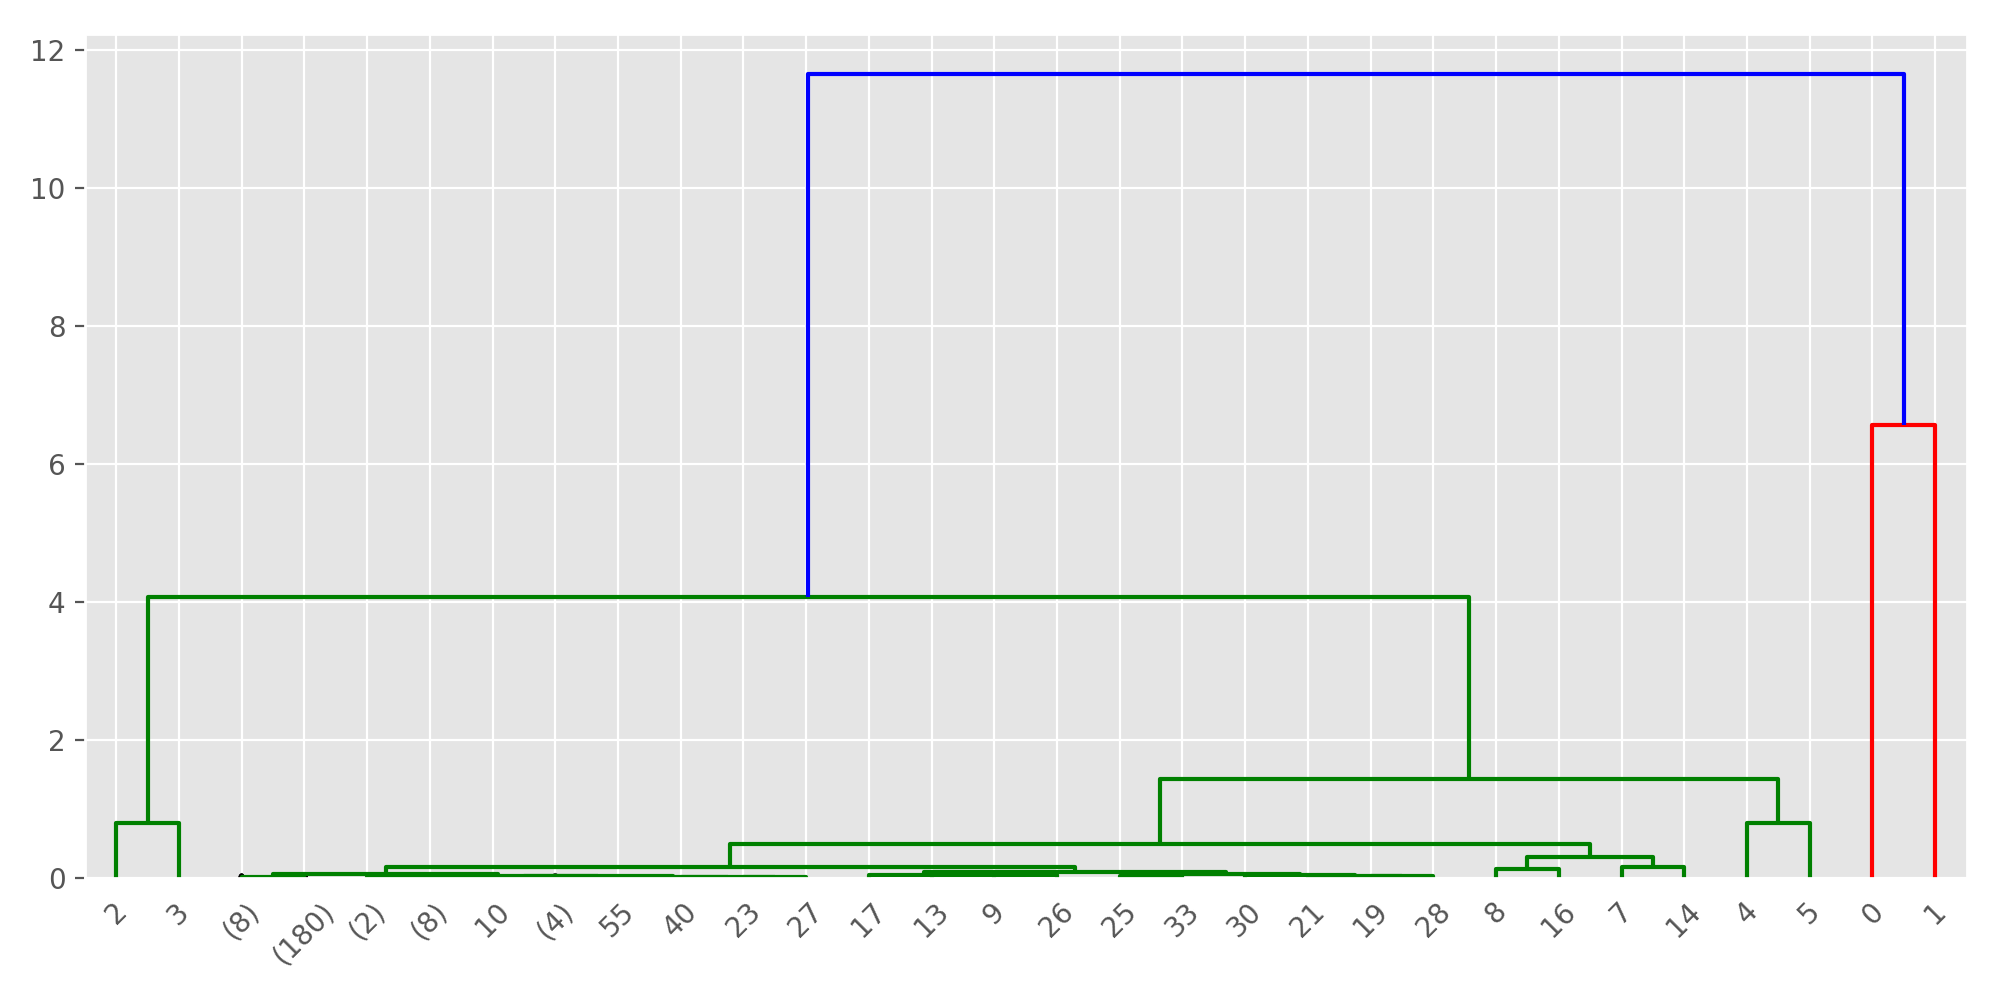
\includegraphics[width=0.9\textwidth]{averagercortado.png}
		\centering
		\caption{Agrupamiento jerárquico.} \label{fig:idf}
	\end{figure}
\end{frame}

\begin{frame}{Variantes como transacciones}
\justifying 
A partir de la base de datos se cálculo las variantes únicas obtenidas dentro del pipeline 29174 de la base se datos y se les asigno un ID a cada una.  \\

Las variantes obtenidas se agruparon por gen y tipo de variante, rango de edad y genero del paciente.
    \begin{table}[H]
	\centering
	\resizebox{10cm}{!}{
	\begin{tabular}{ll|l|l|l|l|l|l|}
		\cline{3-8}
		&   & \textbf{Items} & Tipo de variante & Cigocidad & Rango de edad & Genero & Grupo \\ \hline
		\multicolumn{1}{|l|}{\multirow{2}{*}{\textbf{Transacciones}}} & 1 & BRCA1          & No sinónima      & Het       & (30-40)       & F      & C1      \\ \cline{2-8} 
		\multicolumn{1}{|l|}{}                                        & 2 & RB1            & Stop gain        & Het       & (0-10)        & F      & C5      \\ \hline
	\end{tabular}
}
\caption{Items y transacciones}
\label{tabla:items}
\end{table}

\end{frame}

\begin{frame}{Propuesta de visualización de resultados}
Dashboard
\end{frame}

\section{Conclusiones}
\begin{frame}{Contenido}
    \begin{columns}[onlytextwidth,T]
        \begin{column}{.55\textwidth}
            \tableofcontents[currentsection, sections=1-3]
        \end{column}
        \begin{column}{.60\textwidth}
            \tableofcontents[currentsection, sections=4-]
        \end{column}
    \end{columns}
\end{frame}

\begin{frame}{Conclusiones}

	La utilización de la minería de datos en datos genómicos permite caracterizar e identificar variantes dentro de una población que no ha sido previamente caracterizada.
      
	\bigskip
    El modelo presenta la ventaja de poder utilizar información de diferentes fuentes para realizar un mejor análisis de datos genómicos. 
    \begin{itemize}
    \item Este tipo de análisis son de bajo costo y eficientes.
    \item Puede ser aplicado a otros organismos según la disponibilidad de datos.
    \end{itemize}
  
\end{frame}

\begin{frame}{Trabajo futuro}
\justifying 
 \begin{itemize}
 \justifying 

	\item Aumentar la información  como variantes de exomas y genemas, e información de regional de los pacientes para evaluar la población colombiana.

	\item Desarrollar una base de datos NoSQL para integrar la información procedente de diferentes fuentes y que sea permeable a cambios en el tamaño de la información.
	
	\item Modificar el cálculo de frecuencias del algoritmo Apriori de modo que permita, seleccionar items frecuentes, poco frecuentes e intermedios sin necesidad de que se calcule las asociaciones para todos los ítems. 

\end{itemize}
\end{frame}

\begin{frame}{Publicaciones}
 \begin{figure}[H]
		\centering
		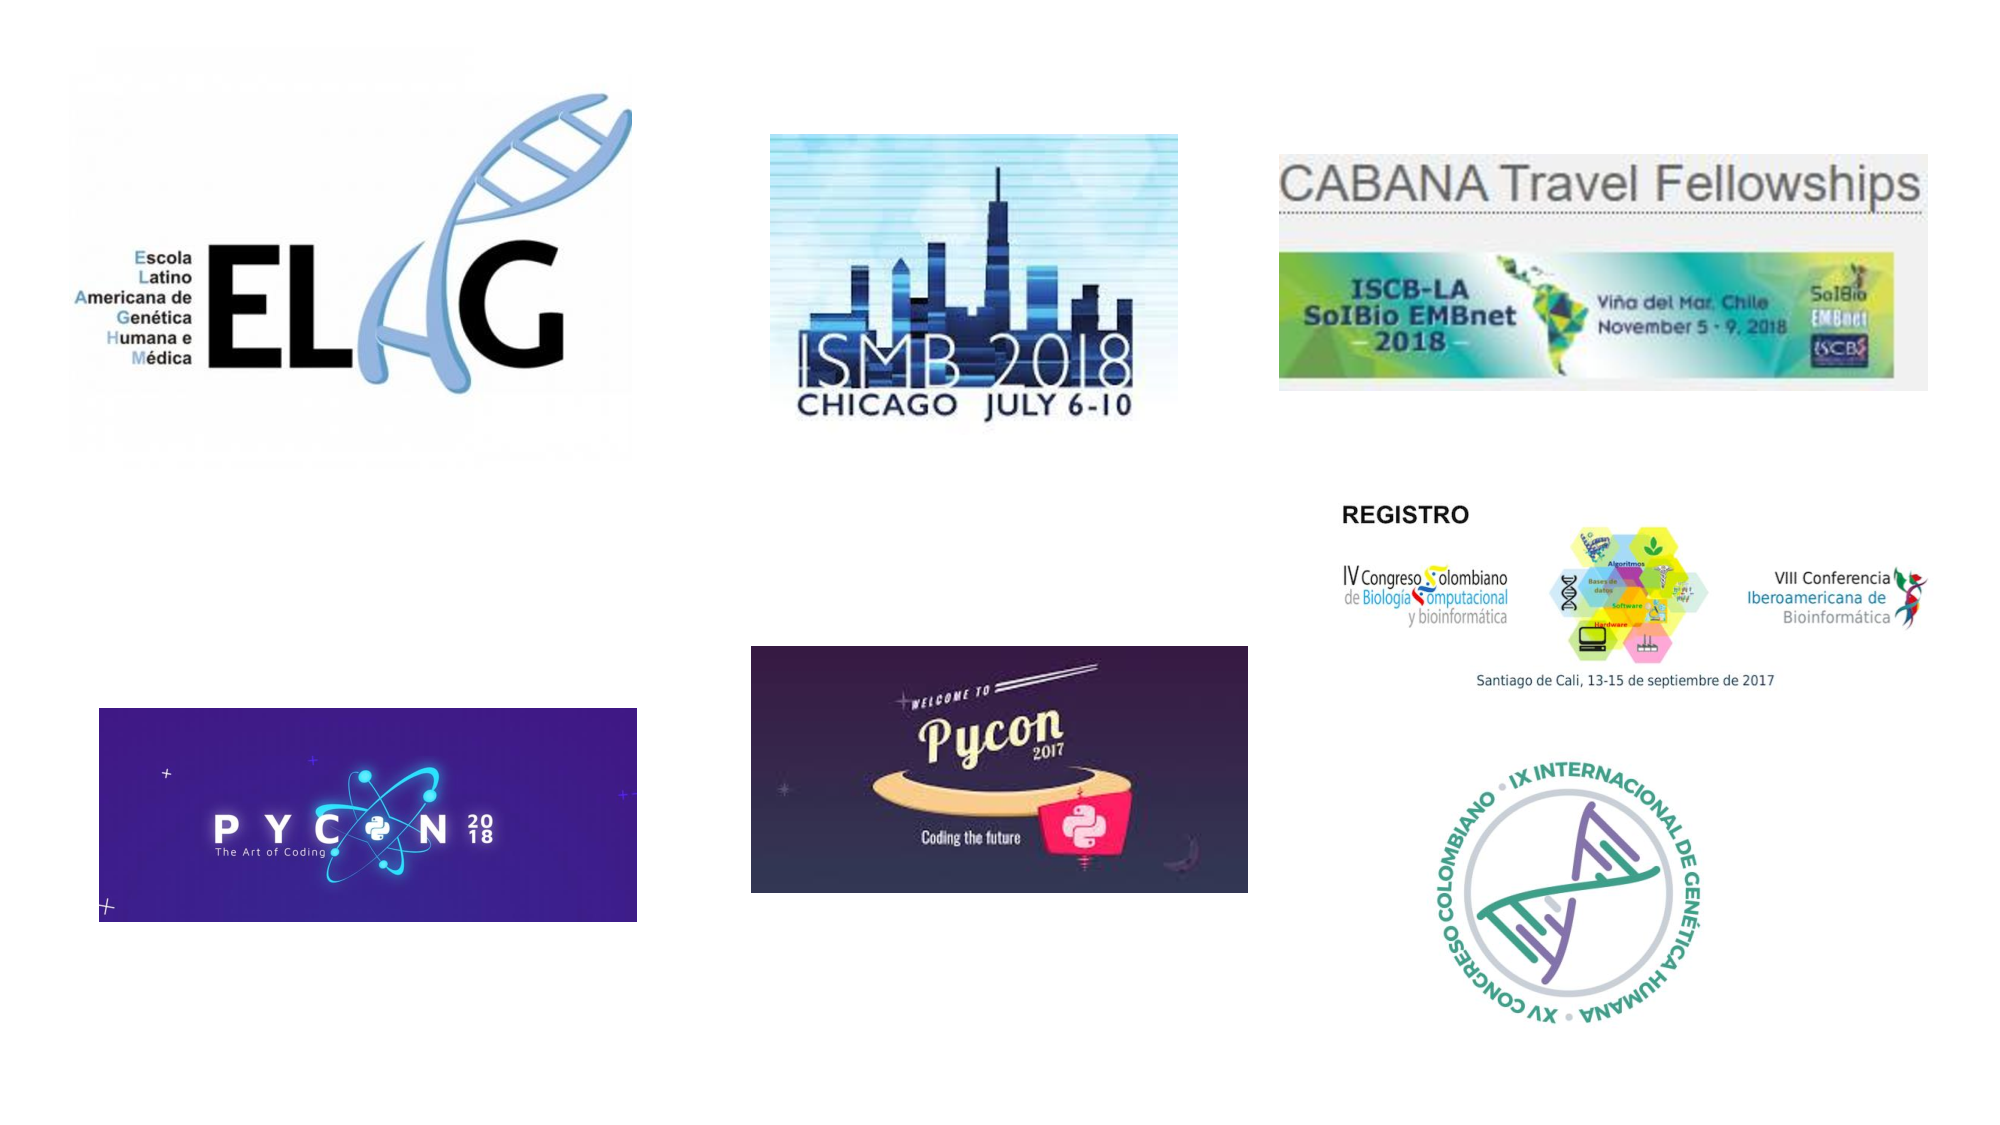
\includegraphics[width=0.8\textwidth]{congresostesis.pdf}
		\centering
		\caption{Presentación en eventos.} \label{fig:p}
	\end{figure}
\end{frame}

\begin{frame}{Agradecimientos}
 \justifying 
    A mi familia que me acompaño en todo este proceso, a Sergio Solano y a Julián Cruz que me apoyaron con sus conocimientos, a la profesora Elizabeth León por dirigir este trabajo y a todo el equipo de Genetix SAS quienes donaron los datos utilizados en este trabajo.
\end{frame}
\begin{frame}{}
  \centering \Large
	{\fontsize{40}{50}\selectfont GRACIAS!}
\end{frame}

\renewcommand{\addcontentsline}[3]{}% Remove functionality of \addcontentsline
\renewcommand{\section}[2]{}% Remove functionality of \section

\begin{frame}[allowframebreaks]
	\frametitle{Referencias}
	\bibliographystyle{apacite}
		\bibliography{library.bib}
\end{frame}

\end{document}
